\chapter{Planung}
\section{Entwürfe}
Da die Entscheidung für das finale Konzept sehr früh gefallen ist, wurde sich darauf geeinigt, dass zwei Gruppenmitglieder dieses Konzept bearbeiten, dafür aber viel tiefer ins Detail gehen. 
Die übrigen zwei Gruppenmitglieder haben jeweils eine eigene Idee behandelt, blieben dabei aber deutlich oberflächlicher. 

Insgesamt sind dabei die drei im Folgenden vorgestellte Konzepte entwickelt worden.

\subsection{Seggway}

\subsection{Weggchair}
Beim Weggchair ist die Namensgebung leider ein wenig misslungen. 
Der Rest vom Konzept wäre mit den vom Lehrstuhl bereitgestellten Materialien recht leicht zu realisieren gewesen.
Deswegen wäre es der Plan B gewesen, falls unser präferiertes Konzept nicht finalisiert werden kann. 

Das Konzept orientiert sich, wie der Name andeuten soll, recht nahe an einem Rollstuhl. 
Die gesamte Elektronik befindet sich in einer Zwischenebene unter der ``Sitzfläche''. 
Gelenkt wird der Weggchair indem sich beide Motoren verschieden schnell drehen. 

Wie in der Skizze (Abb.~\ref{bild:weggchair}) zu sehen, ist das ``Stützrad'' eher eine ``Stützkugel'', die in alle Richtungen über den Boden gleiten kann. 
Statt einer Kugel wäre auch eine oder zwei drehbar gelagerte Rollen denkbar gewesen, ähnlich wie bei einem Einkaufswagen oder natürlich dem Original. 

Da die verwendeten DC-Motoren unter Volllast über 7000 Umdrehungen schaffen, dafür aber weniger Drehmoment haben wäre, wie in der finalen Idee, ein Planetengetriebe innerhalb der großen Räder zum Einsatz gekommen. 

Das Ei wäre wäre beim Weggchair an der Stelle befestigt, wo normalerweise der Rollstuhlfahrer sitzt. Dafür wäre eine Federung und Halterung an dieser Stelle gewesen. Vermutlich wäre ein mit Watte oder einem ähnlichen elastischen, polsternden Material ausgestatteter Eierbecher zum Einsatz gekommen.

\begin{figure}[!ht]
	\centering
	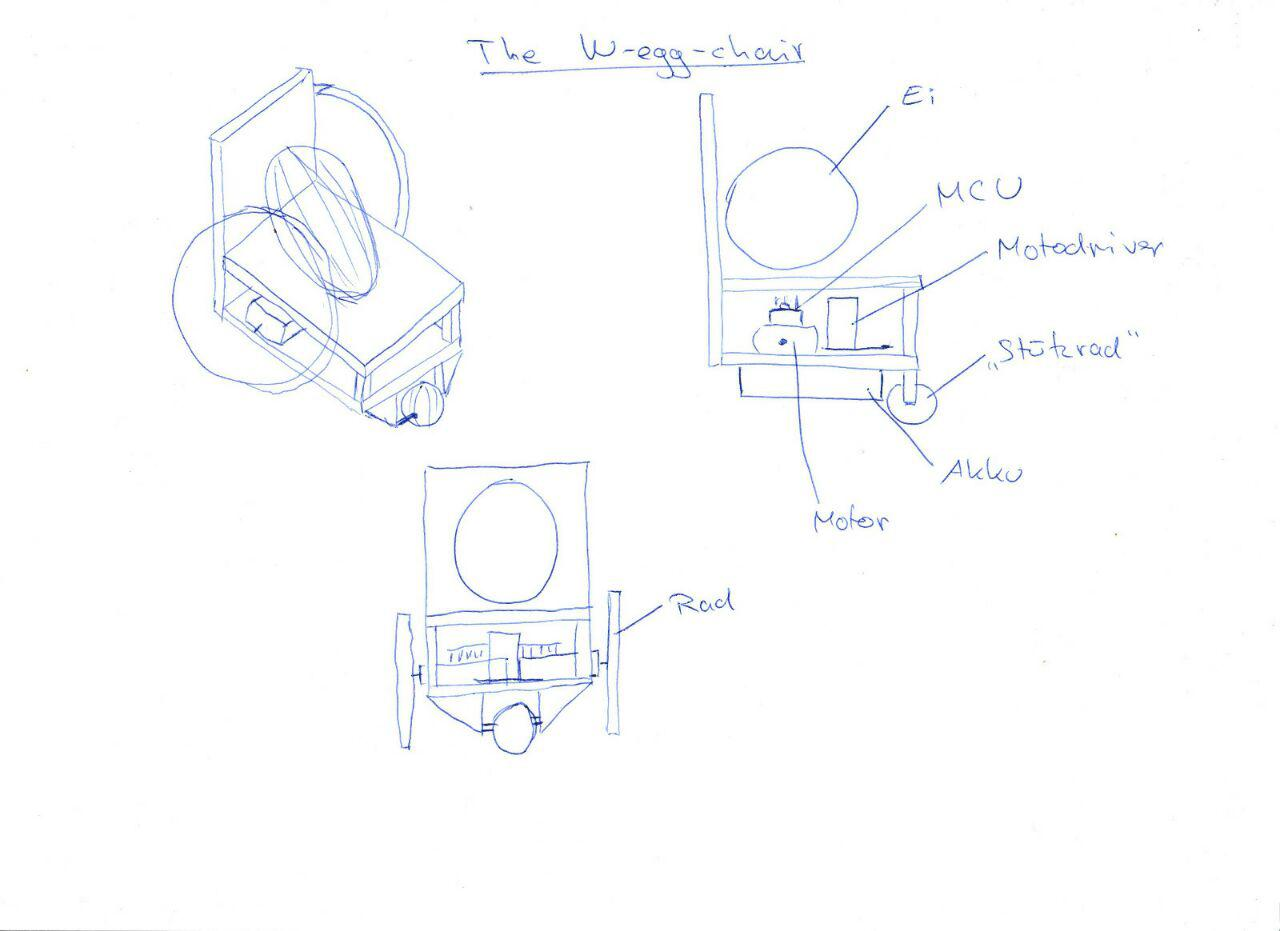
\includegraphics[width=\textwidth]{bilder/weggchair.jpg}
	\caption{Skizze Weggchair}
	\label{bild:weggchair}
\end{figure}


\subsection{TEGGLA}
Da sich die nächsten drei Kapitel nur mit dem finalen Konzept auseinandersetzen, wird an dieser Stelle nur ganz kurz auf das Konzept des TEGGLA (Abb.~\ref{bild:tegglaskizze}) eingegangen, damit die nachfolgenden Kapitel nachvollziehbar sind. 

Das besondere Feature beim TEGGLA sind die omnidirektionalen Räder, auch Mecanum bezeichnet, die neben dem normalen Vorwärtsfahren auch Seitwärtsbewegungen und Rotation zulassen. 
Diese drei Freiheitsgrade lassen sich auch beliebig kombinieren. 
Dadurch ist in der Ebene jede denkbare Richtung befahrbar. Dazu sind allerdings vier Motoren notwendig. 

Ergo wächst die Elektronikteileliste wie folgt: Für die zwei Extramotoren wird eine zusätzliche H-Brücke benötigt. 
Leider hat das bereitgestellte ESP-8266 nicht genug Pins für die zusätzliche Elektronik, weswegen zum ESP-32 upgegraded werden musste. 

Es folgen noch viel mehr Details, aber um die folgenden Kapitel zu verstehen muss noch gesagt werden, dass der TEGGLA in der Entwicklungsphase noch Omni-Move hieß. Beide Namen sind im Folgenden also synonym. 

\begin{figure}[!ht]
	\centering
	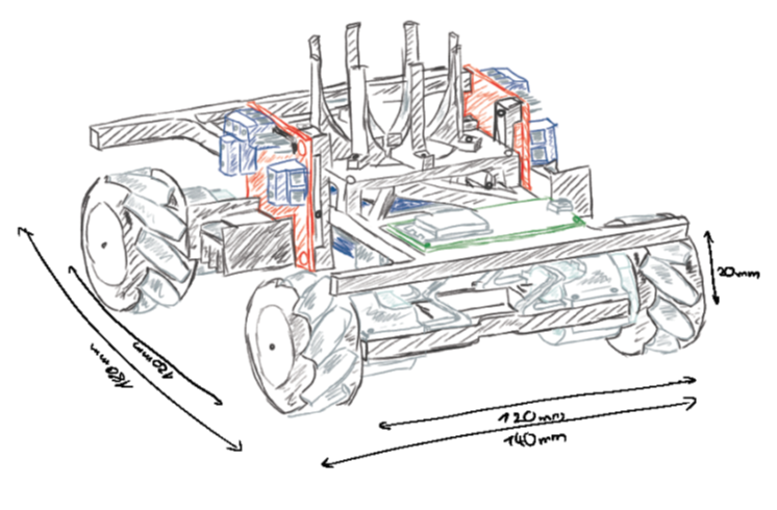
\includegraphics[width=\textwidth]{bilder/tegglaskizze.png}
	\caption{Skizze TEGGLA}
	\label{bild:tegglaskizze}
\end{figure}


\section{Morphologischer Kasten}
Mithilfe des Morphologischen Kasten (Abb.~\ref{bild:morphkasten}) lassen sich die benötigten Komponenten auf eine einfach ersichtliche Weise vergleichen.
\begin{figure}[!ht]
	\centering
	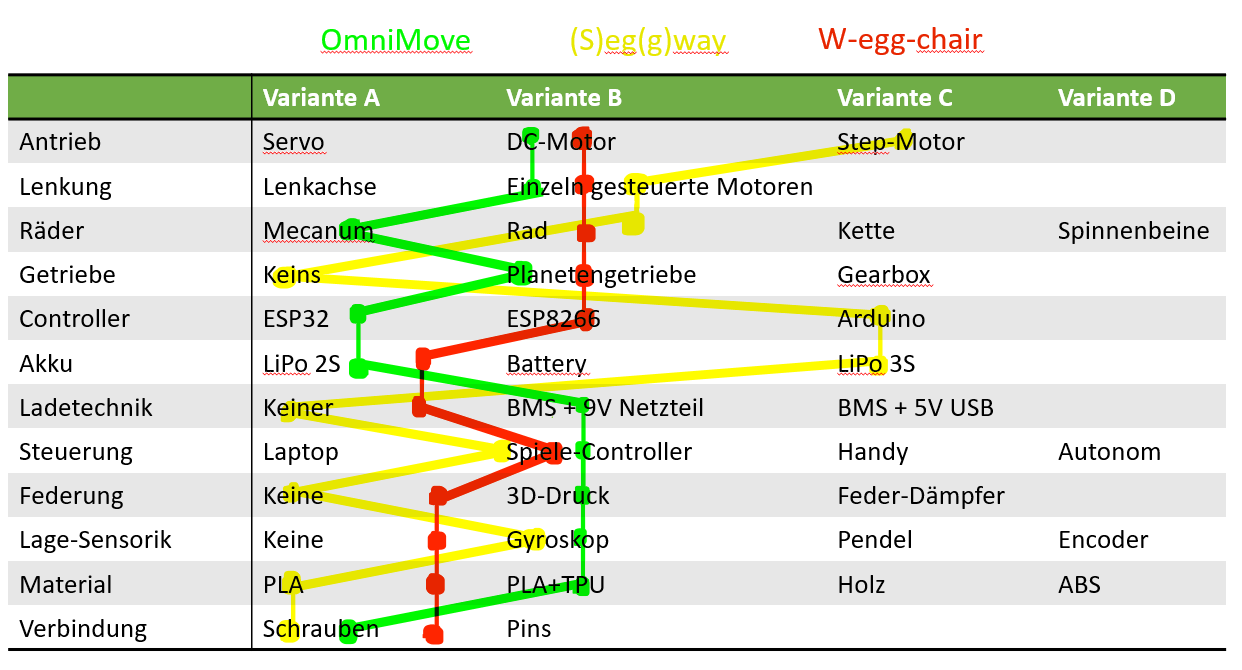
\includegraphics[width=\textwidth]{bilder/morphkasten.png}
	\caption{Morphologischer Kasten}
	\label{bild:morphkasten}
\end{figure}

\section{Online Bestellungen}
Um das Fahrzeug nach dem Praktikum behalten zu können, war eine Voraussetzung, dass nur Teile verbaut werden, die nicht Eigentum des Lehrstuhls sind.
Aus diesem wurden die nötigen Bauteile bei unterschiedlichen Onlineshops herausgesucht und bestellt.
Hierbei fiel die Entscheidung auf Pollin, einem deutschen Elektronik Händler und AliExpress, einem chinesischen Großhändler.
In der ursprünglichen Planung wurden die Kosten pro Fahrzeug auf circa \EUR{20} -- \EUR{25} überschlagen.
In der finalen Bestellung beliefen sich die Kosten auf insgesamt etwa \EUR{32}.

Siehe Tabelle~\ref{table:Kosten} für eine genaue Aufteilung der Kosten.
\begin{table}[!ht]
	\centering
\begin{tabular}{lcccc}
	Artikel & Stk & \euro/Stk & \euro{} & Laden\\
	\midrule[2pt]
	Netzteil 9V 1A & 1 & 0,95 & 0,95 & Pollin\\
	\midrule
	DC Motor & 4 & 0,95 & 3,80 & Pollin\\
	\midrule
	2S LiPo & 1 & 9,95 & 9,95 & Pollin\\
	\midrule
	XT60 5er Satz & 0,5 & 1,8 & 0,90 & AliExpress\\
	\midrule
	ESP32 & 1 & 3,77 & 3,77 & AliExpress\\
	\midrule
	2s BMS & 1 & 0,89 & 0,89 & AliExpress\\
	\midrule
	Kabelset 20cm & 0,5 & 3,30 & 1,65 & AliExpress\\
	\midrule
	Kabelset F -- F 10cm & 0,5 & 0,68 & 0,34 & AliExpress\\
	\midrule
	Gyroskop & 1 & 0,93 & 0,93 & AliExpress\\
	\midrule
	H-Brücken & 2 & 1,17 & 2,34 & Bestand\\
	\midrule
	Filament \textit{[kg]} & 0,05 & 20,00 & 1,00 & Bestand\\
	\midrule
	Schrauben + Muttern \textit{[Set]} & 1 & 1,00 & 1,00 & Bestand\\
	\midrule
	Motorkabel & 1 & 0,50 & 0,50 & Bestand\\
	\midrule
	Versandkosten AliExpress & 0,25 & 9,00 & 2,25 & \\
	\midrule
	Versandkosten Pollin & 0,25 & 5,00 & 1,25 & \\
	\midrule
	\midrule
	 &  & Total & \EUR{31,52} & \\
\end{tabular} 
\caption{Kostenübersicht} 
\label{table:Kosten}
\end{table} 

\section{Verwendete Technologien}

\subsection{Git}
\subsection{Creo}
Bei der CAD-Software standen mehrere unterschiedliche Programme unterschiedlicher Hersteller zur Auswahl.
Diese waren ``Catia'' von Dassault Systemes, ``Sketchup'' von Trimble Inc., ``Blender'' von Blender Foundation
\subsection{PlatformIO}
Die Wahl der Entwicklungsumgebung fiel auf Visual Studio Code mit PlatformIO, anstelle von der in der Vorlesung vorgestelleten Arduino IDE.

Mit der extremen Erweiterbarkeit von VSCode ist hier die Programmierung einfacher und fehlerfreier durchzuführen, da in Arduino IDE nur bedingtes Syntax-checking vorhanden ist.

Durch PlatformIO stellt sich Einbingen von externen Bibliotheken ebenfalls als Leichtigkeit heraus.
Desweiteren ist hier die Unterstützung von einer Vielzahl von MicroControllern bereits integriert.